
This category of backgrounds includes processes with a single leptonic \W~decay, giving rise to one lepton and \met\ from a single neutrino.
As a result, the \mt\ variable, constructed from the lepton and the \met, exhibits a kinematic edge at $\mt \sim \mW$. The main contributors
to this background are \ttlj, \wjets\ and single top, though in the latter case there is a contribution from \tw\ that can give rise to two leptons. 
As shown in Figure.~\ref{fig:mtsinglelepcomp} (left), these backgrounds exhibit a similar \mt\ shape and are thus combined into a single 
background estimate. 

It should be underlined that single lepton events entering the signal sample are in the far \mt~tail for these processes
and contribute mainly due to the \met\ resolution that smears the \mt\ peak, particularly in the presence of multiple jets. 
Since these types of effects are challenging to model in simulation, the background estimate for this category of processes is cross checked 
in a control sample in data. The control sample is obtained by applying the full selection criteria with the exception of the b-tagging requirement, 
that is reversed, vetoing events with b-tagged jets. The b-tag veto greatly reduces the contamination from \ttbar, which is particularly important
in the case of \ttll\ which otherwise populates the \mt\ tail. The resulting sample is dominated by \wjets\ events. The derivation of the background 
estimate in this control sample serves to validate the method. 
In addition, the level of agreement between the prediction and the data in the \mt\ tail provides an estimate of the systematic uncertainty for this
background prediction. 

\begin{figure}[hbt]
  \begin{center}
	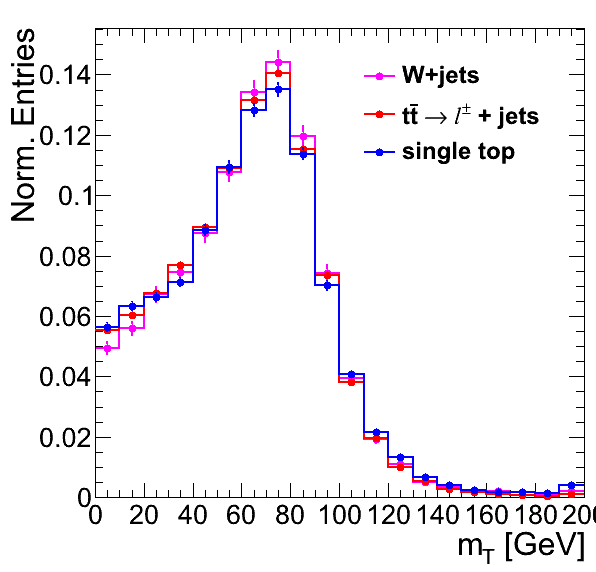
\includegraphics[width=0.5\linewidth]{plots/mt_singlelepcomp_full.png}%
        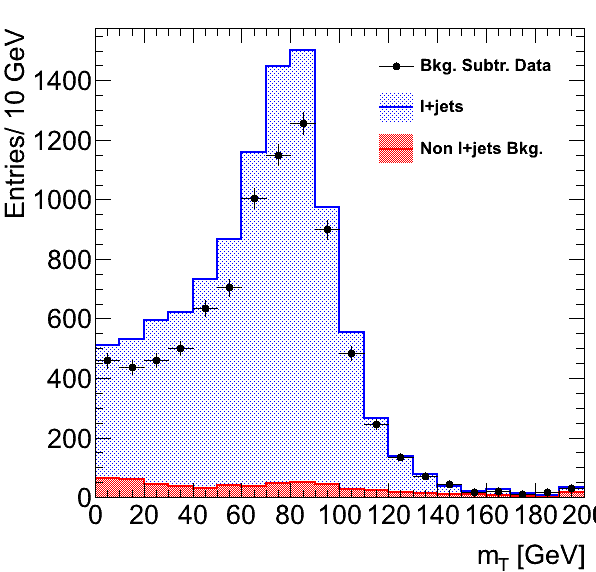
\includegraphics[width=0.5\linewidth]{plots/mt_bkgsubt_bveto_met50.png}
	\caption{
	  \label{fig:mtsinglelepcomp}%\protect 
          Monte Carlo comparison of the shapes (left) of the \mt\ distribution for the main background processes containing a single leptonic \W\ decay (left).
          The \mt\ shape for \ttlj, \wjets\ and single top are similar and thus combined into a single background estimate. Comparison of the MC 
        prediction (right) for single lepton processes (blue) and the data after subtracting the non-single lepton background MC prediction (also shown in red). 
        The \mt\ distribution in MC is scaled to the data in the \mt\ peak region ($60-100~\GeV$). Since the control sample is dominated by $\Wfourj$ events, 
        the MC is not expected to provide an estimate of the overall normalization to better than the $\sim 15\%$ difference observed.}
  \end{center}
\end{figure}

The single lepton background contribution to the tail of the \mt\ is derived from MC and normalized to the data in the \mt\ peak region, defined by the 
range $60 < \mt \le 100~\GeV$. In particular, the total yield for the combination of the single lepton + jets samples in MC satisfying $60 < \mt \le 100~\GeV$
is scaled to match the entries in data satisfying the same \mt\ requirement. The data is corrected for the expected contamination from non-single 
lepton + jets processes, which is obtained from MC. The derivation of this MC to data scale factor is shown in Figure.~\ref{fig:mtsinglelepcomp} (right), where the 
contribution from non-single lepton + jets processes in the \mt\ peak is also shown to be small. 
Scaling to the data yield in the \mt\ peak largely reduces the dependence on the \ttbar\ cross section and cancels systematic uncertainties associated with
effects such as the luminosity, selection efficiencies, etc$\dots$
 

\begin{figure}[!ht]
  \begin{center}
	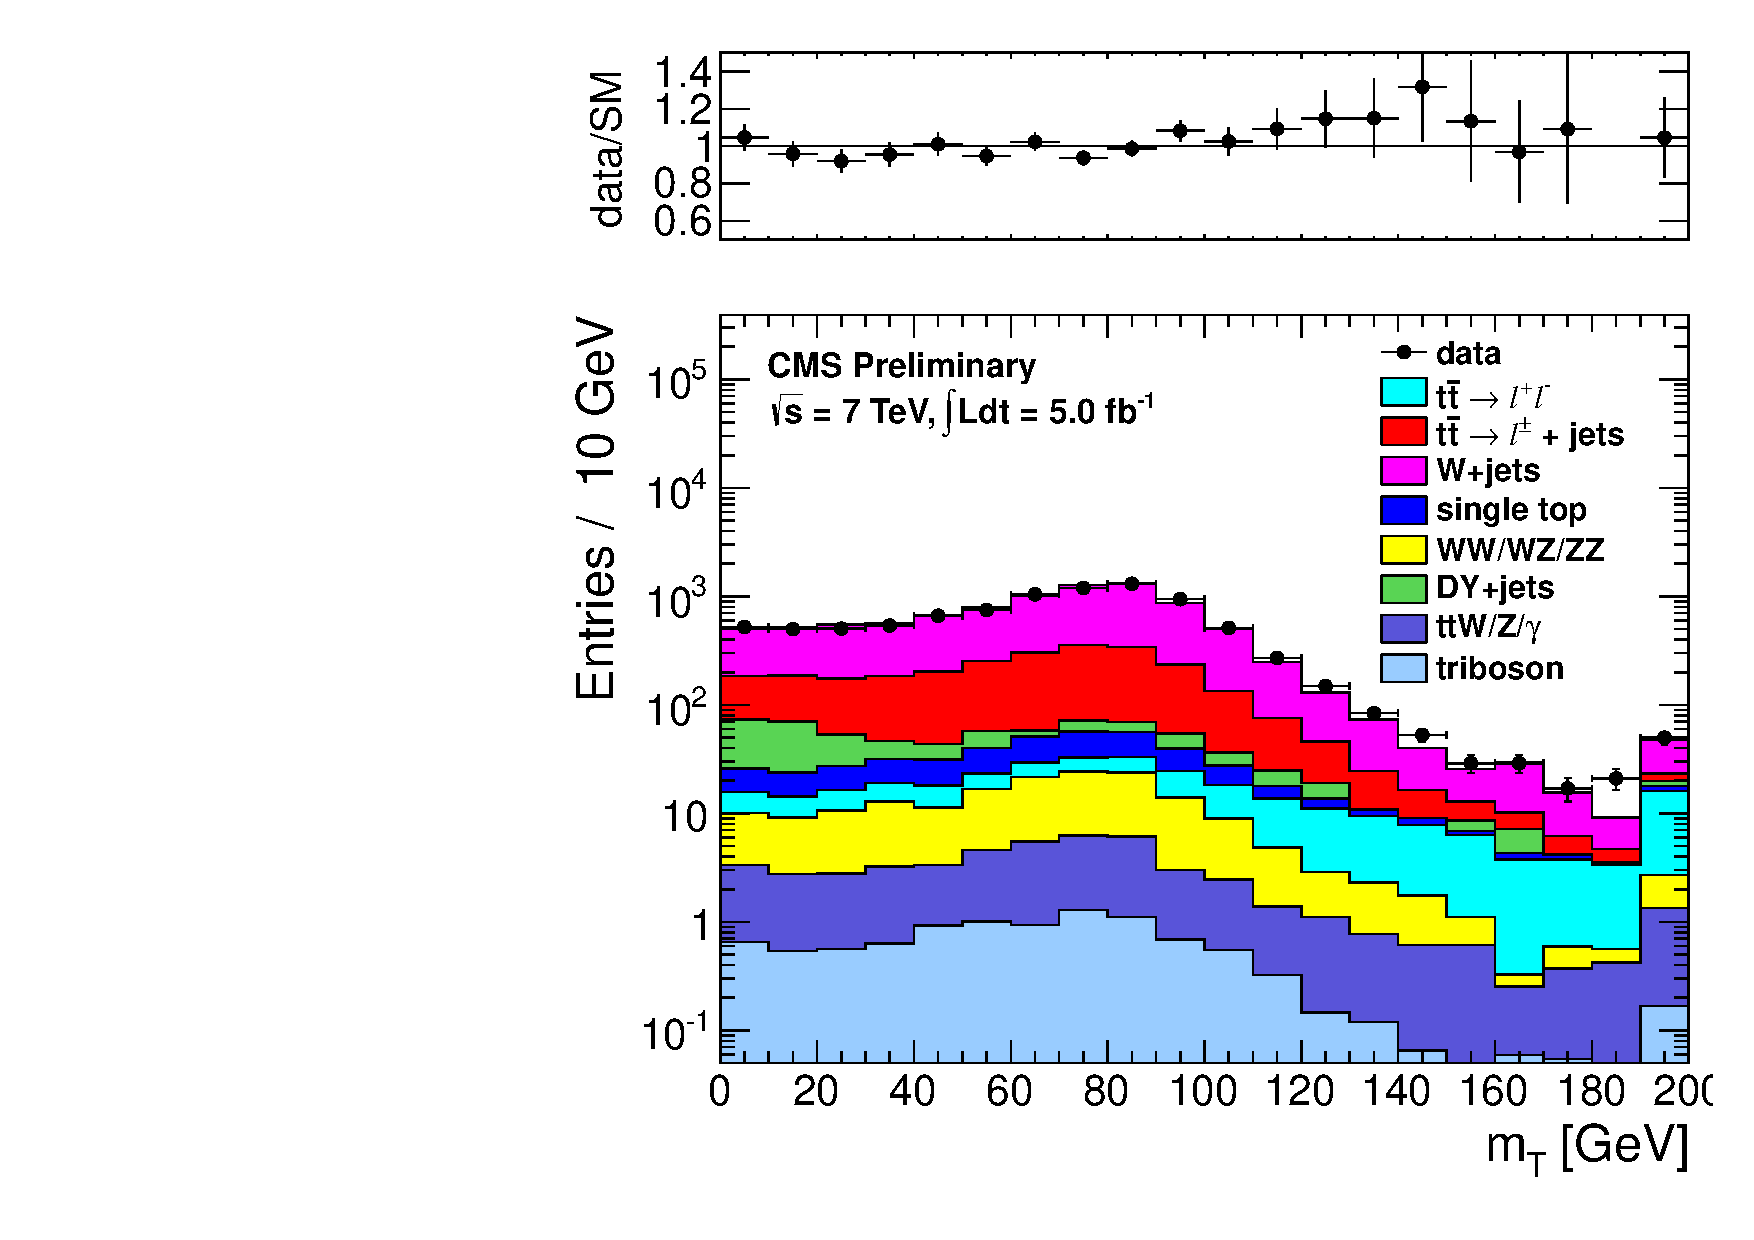
\includegraphics[width=0.5\linewidth]{plots/mt_met50_bveto.pdf}%
        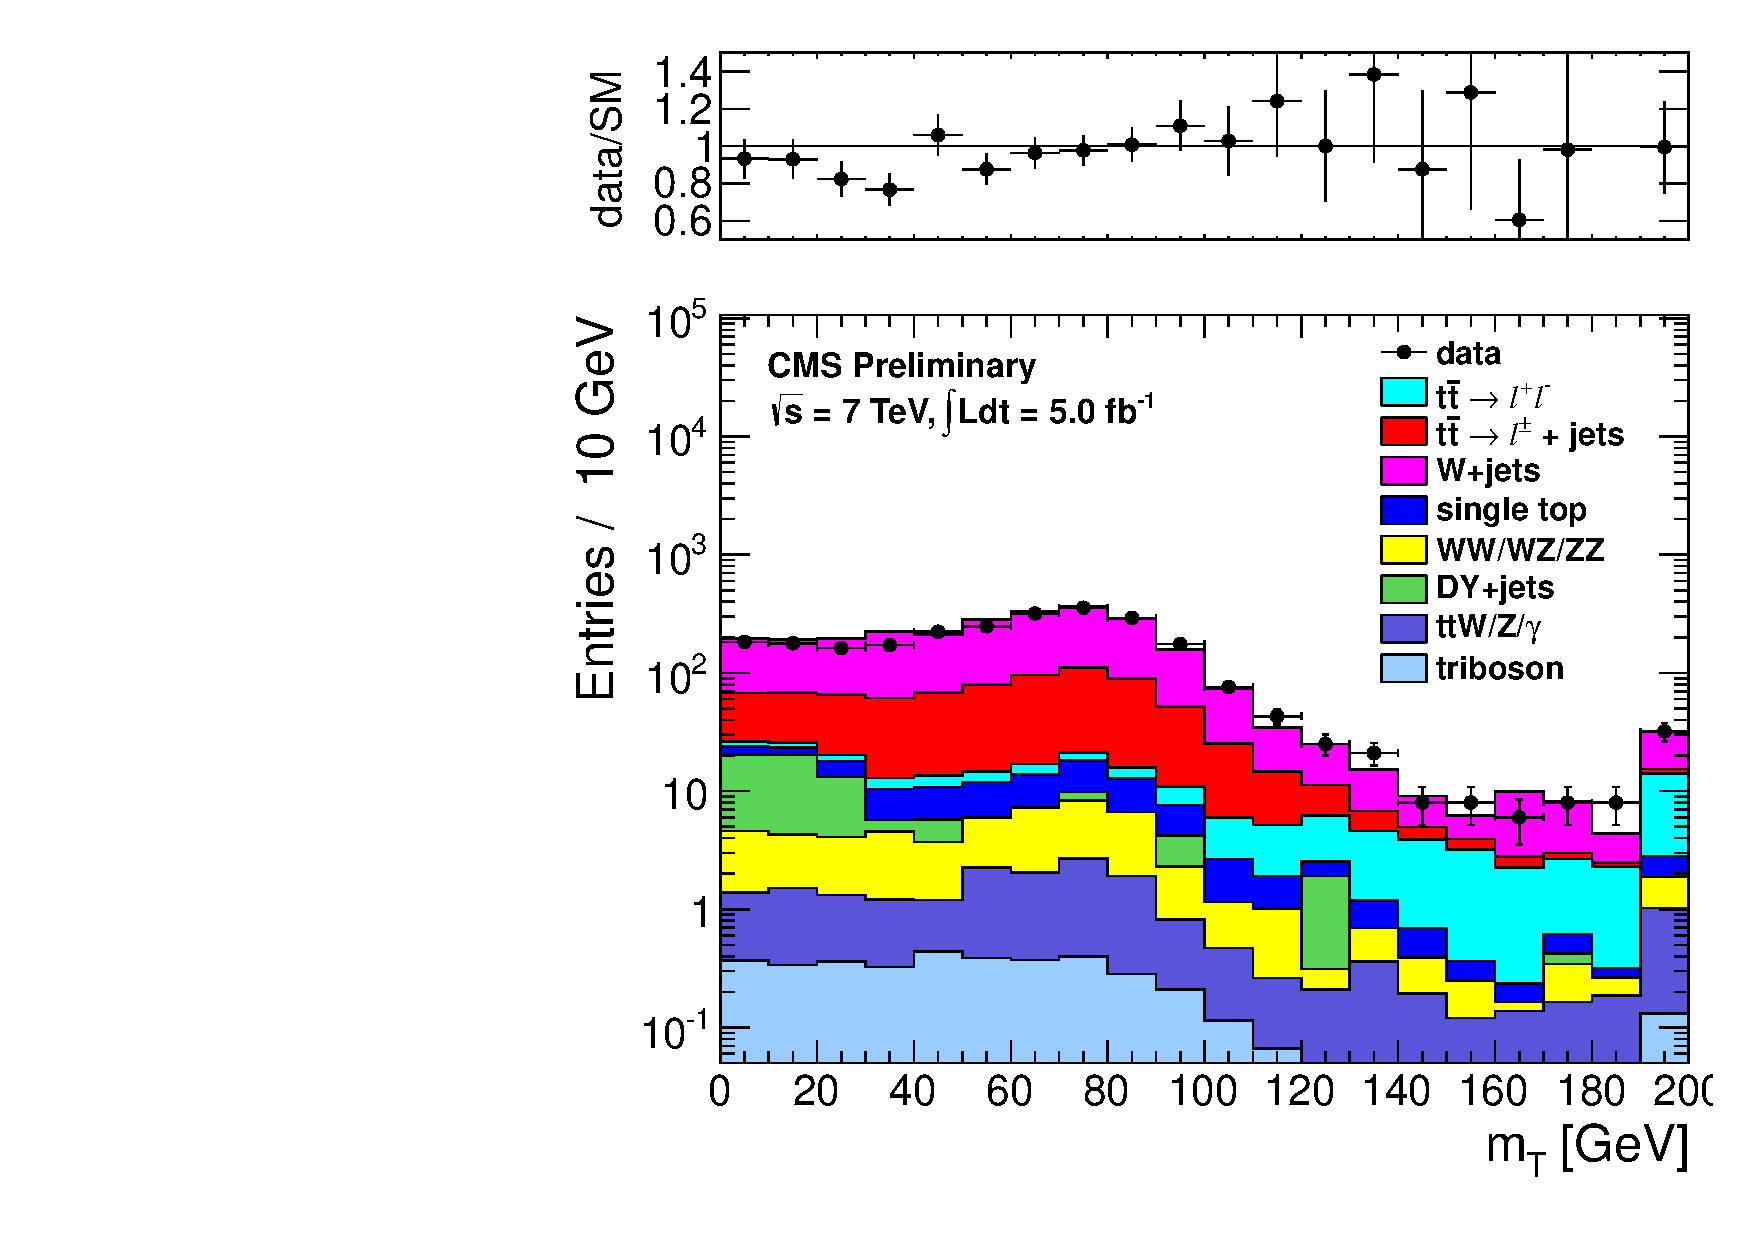
\includegraphics[width=0.5\linewidth]{plots/mt_met100_bveto.pdf}
	\caption{
	  \label{fig:mtbveto}%\protect 
          Comparison of data and MC in the b-veto sample after scaling the single lepton samples in the \mt\ peak region ($60-100~\GeV$) for two \met\ requirements
          $\met>50~\GeV$ (left) and $\met>100~\GeV$ (right). The simulation shows reasonable agreement with the data both in the peak and the \mt\ tail, as can also 
          be seen the ratios.}  
      \end{center}
\end{figure}


\begin{figure}[!hb]
  \begin{center}
        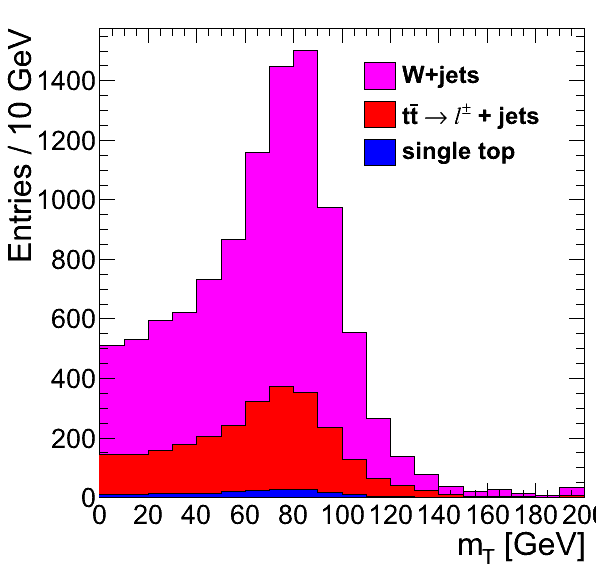
\includegraphics[width=0.5\linewidth]{plots/mt_singlelepcomp_full_stack.png}%
	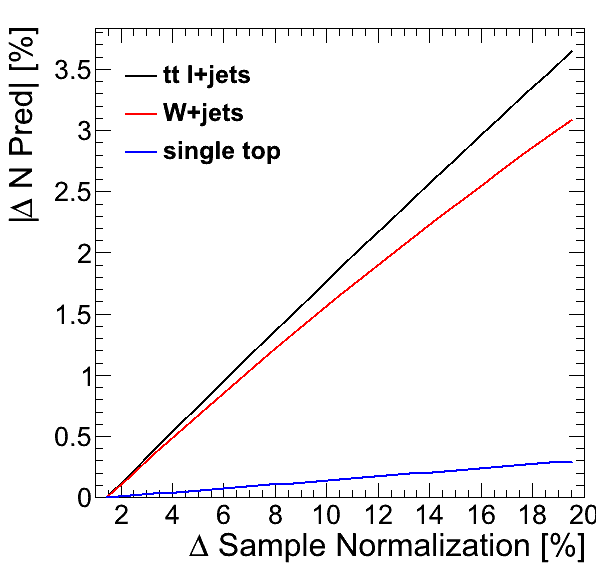
\includegraphics[width=0.5\linewidth]{plots/bkg_comp_err_mt_met100.png}
	\caption{
	  \label{fig:mtsamplecomperr}%\protect 
          Stacked plot (left) showing the relative sample composition in MC for the main single lepton + jets components, \ttlj, \wjets\ and single top
          sample for the b-veto control selection. Note no scalings are applied and the $\met>50~\GeV$ is shown. Percent change in the total single lepton + jets
          background prediction for variations in the normalization of each single lepton + jets background component (right). Each sample is varied independently and the
          full background prediction is performed.}
      \end{center}
\end{figure}


\begin{table}[!ht]
\begin{center}
\begin{tabular}{c|c|c}
\hline
Sample                   &   $\met>50~\GeV$  &   $\met>100~\GeV$  \\
\hline
\hline
Lepton + Jets Prediction           & $88 \pm 12$  & $38 \pm 8$   \\
Data in Signal Region               & $106 \pm 13$ & $40 \pm 8$   \\
\hline
Data/MC Closure                     & $1.20 \pm 0.22$ & $1.03 \pm 0.30$   \\
\hline
\end{tabular}
\caption{Summary of closure test in b-veto control sample for two values of the \met\ requirement. The closure serves to estimate the systematic uncertainty for 
  the prediction of the single lepton + jets background.\label{tab:ljetsclosure}}
\end{center}
\end{table}

Figure~\ref{fig:mtbveto} shows a comparison of the \mt\ distribution in data and MC in the b-veto control sample for two values of the \met\ cut after scaling 
the single lepton contribution to the \mt\ peak region. The simulation models the \mt\ distribution in data reasonably well. Table~\ref{tab:ljetsclosure} shows 
a comparison of the single lepton + jets prediction and the data in the $\mt>150~\GeV$ region. The prediction and the data are in agreement
within the statistical uncertainty, which is $30 \%$ for the $\met>100~\GeV$ case. No correction is necessary given the agreement observed and the uncertainty 
serves as an estimate of the systematic uncertainty on the lepton + jets background. It may be noted that the $30\%$ uncertainty applies to the lepton + jets
background, which constitues $15\%$ of the sample. The resulting uncertainty on the total background is $\approx5\%$, within our uncertainty budget of $\approx10\%$.

Given the similarities in the shapes of the \mt\ distributions for the various samples, the resulting dependence on the sample composition is small. 
Figure.~\ref{fig:mtsamplecomperr} shows the \mt\ distribution for the single lepton + jets components in MC. The distribution on the right shows the impact of 
varying the relative sample composition on the total single lepton + jets prediction. In this study, each component is varied independently by up to $20\%$ and 
the corresponding change on the prediction is at the level of a few percent and therefore negligible compared to the statistical uncertainty of the closure test. 
It should be noted that despite differences in the \mt\ shape for the various single lepton + jets processes, expected for example due to differences in the \pt\ of the \W, 
this test provides a check for the impact of reconstruction effects, such as the \met\ resolution, that are the dominant contributors to the tail of the \mt\ and similar 
for the \ttlj\ and \wjets\ processes. 



